\documentclass{article}
\usepackage[a4paper,margin=1in]{geometry}
\usepackage{amsmath, amsfonts, amssymb, amstext, mathtools, stmaryrd, textcomp, xcolor, graphicx, tikz}
\usepackage[hidelinks]{hyperref}
\usetikzlibrary{automata, positioning, arrows, trees}
\tikzset{->,>=stealth,
every state/.style={thick, fill=gray!10}, 
initial text=$ $,
}
\newcommand{\e}{\varepsilon}
\newcommand{\s}{\Sigma}
\newcommand{\g}{\Gamma}
\newcommand{\so}{\rightarrow}
\newcommand{\str}{\texttt}
\newcommand{\newp}{\\[2mm]}
\newcommand{\defeq}{\coloneqq}

\title{Homework 04}
\author{Aaron Wang}
\date{February 21 2025}

\begin{document}
\maketitle
\begin{enumerate}
    \item \textbf{Arithmetic expressions}. Consider the grammar $G_4$ (page 105) for arithmetic expressions, with start symbol $E$:
    \begin{align*}
        & E \rightarrow E \: \str{+} \: T \: | \: T\\
        & T \rightarrow T \: \str{*} \: F \: | \: F\\
        & F \rightarrow \str{(}E\str{)} \: | \: \str{a} \: | \: \str{b} \: | \: \str{c}
    \end{align*}
    \begin{enumerate}
        \item [(a)][cf. Exercise 2.1] Give derivations for the following strings. You may write them either as a sequence of rewrites $(E \implies \cdots)$ or as a tree.
        \begin{enumerate}
            \item \str{a + b + c}
            \item \str{a * b + c}
            \item \str{a * (b + c)}
        \end{enumerate}
        \begin{figure}[ht]
\centering
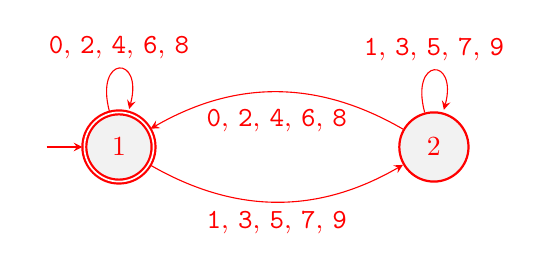
\begin{tikzpicture}
\color{red}
    \node[state, initial, accepting] (q1) {1};
    \node[state, right of=q1, xshift=3cm] (q2) {2};
    \draw (q1) edge[loop above] node[]{\str{0}, \str{2}, \str{4}, \str{6}, \str{8}} (q1)
    (q2) edge[loop above] node[]{\str{1}, \str{3}, \str{5}, \str{7}, \str{9}} (q2)
    (q2) edge[bend right] node[below, yshift=-0.1cm]{\str{0}, \str{2}, \str{4}, \str{6}, \str{8}} (q1)
    (q1) edge[bend right] node[below]{\str{1}, \str{3}, \str{5}, \str{7}, \str{9}} (q2);
\end{tikzpicture}
\end{figure}
        \item [(b)]Modify $G_4$ to allow an exponentiation operator $\uparrow$.
        \begin{itemize}
            \item It should have \textit{higher precedence} than multiplication; that is, in the derivation of the string \str{a * b} $\uparrow$ \str{c}, there should be a nonterminal that rewrites to \str{b} $\uparrow$ \str{c}, and there should not be a nonterminal that rewrites to \str{a * b}.
            \item It should be (unlike \str{*} and \str{+}) \textit{right-associative}; that is, in the derivation of the string\\ \str{a} $\uparrow$ \str{b} $\uparrow$ \str{c}, there should be a nonterminal that rewrites to \str{b} $\uparrow$ \str{c}, and there should not be a nonterminal that rewrites to \str{a} $\uparrow$ \str{b}.
        \end{itemize}
        \begin{figure}[ht]
\centering
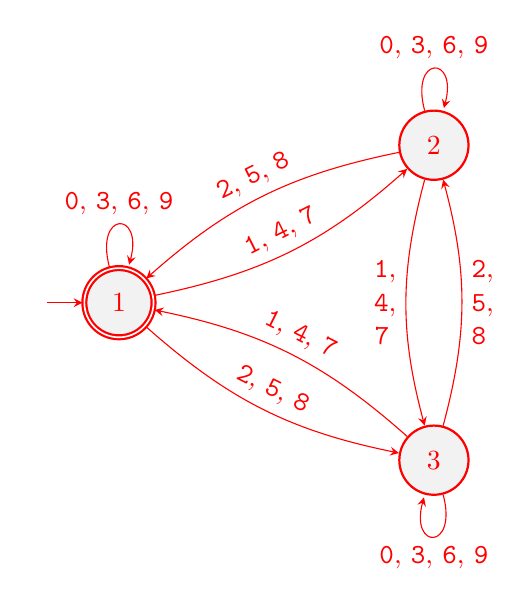
\begin{tikzpicture}
\color{red}
    \node[state, initial, accepting] (q1) {1};
    \node[state, right of=q1, xshift=3cm, yshift=2cm] (q2) {2};
    \node[state, right of=q1, xshift=3cm, yshift=-2cm]  (q3) {3};
% go forward one node  
    \draw (q1) edge[bend right=15] node[sloped, above]{\str{1}, \str{4}, \str{7}} (q2)
    (q2) edge[bend right=15] node[left, align=center]{\str{1},\\ \str{4},\\ \str{7}\:} (q3)
    (q3) edge[bend right=15] node[sloped, above]{\str{1}, \str{4}, \str{7}} (q1)
% go back one node     
    (q1) edge[bend right=15] node[sloped, above]{\str{2}, \str{5}, \str{8}} (q3)
    (q3) edge[bend right=15] node[right, align=center]{\str{2},\\ \str{5},\\ \str{8}\;} (q2)
    (q2) edge[bend right=15] node[sloped, above]{\str{2}, \str{5}, \str{8}} (q1)
% looping nodes
    (q1) edge[loop above] node[above]{\str{0}, \str{3}, \str{6}, \str{9}} (q1)
    (q2) edge[loop above] node[above]{\str{0}, \str{3}, \str{6}, \str{9}} (q2)
    (q3) edge[loop below] node[below]{\str{0}, \str{3}, \str{6}, \str{9}} (q3)
    ;     
\end{tikzpicture}
\end{figure}
    \end{enumerate}
    \item Write both a PDA and a CFG for the language (page 80):
    \[
    C = \big\{w \in \{0, 1\}^* | w\text{ has an equal number of \str{0}s and \str{1}s}\big\}.
    \]
    Please include a brief explanation of why they work. (If you design a PDA and then convert it to a CFG, your explanation for the CFG can simply be, ``I converted my PDA to a CFG,'' and similarly if you convert a CFG to a PDA.)\newp
    \textcolor{red}{
    The intuition for the following CFG is this. We need to design a CFG that accepts only balanced strings and every balanced string. This CFG clearly only accepts balanced strings as it only adds \str{0} and \str{1} simultaneously. 
    Now for the other half, a balanced string must fall into at least one of two categories. 
    The first is that $w=\str{0}x\str{1}$ or $w=\str{1}x\str{0}$ s.t. $x$ is a balanced string (it is composed of a balanced substring wrapped by \str{0} and \str{1}). 
    The other is $w=xy$ s.t. $x$, $y$ are balanced strings (It is a concatenation of two balanced substrings).
    Both of these cases are covered by the following CFG.\newp
    CFG for C with starting state $S$.
    \begin{align*}
    S &\rightarrow \str{0}S\str{1} \:|\: \str{1}S\str{0} \:|\: SS \:|\: \e
    \end{align*}
    The intuition for the following PDA is this. At each occurence of a character, we either pop the opposing character off the stack (if possible) or we add the current character onto the stack. This way, the stack will always be empty\footnote{airquotes because it will contain the \$ which signifies empty stack.} if and only if an equal amount of occurences of each character exist.\newp
    \begin{figure}[h]
    \centering
    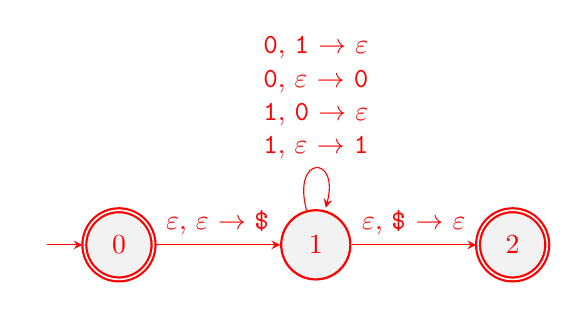
\begin{tikzpicture}
    \color{red}
        \node[state, initial, accepting] (q0) {0};
        \node[state, xshift=2.5cm] (q1) {1};
        \node[state, xshift=5cm, accepting] (q2) {2};
        \draw
        (q0) edge[] node[above]{$\e$, $\e$ $\rightarrow$ \str{\$}} (q1)
        (q1) edge[loop above] node[above, align=center]{
            \str{0}, \str{1} $\rightarrow$ $\e$\\
            \str{0}, $\e$ $\rightarrow$ \str{0}\\
            \str{1}, \str{0} $\rightarrow$ $\e$\\
            \str{1}, $\e$ $\rightarrow$ \str{1}
        } (q1)
        (q1) edge[] node[above]{$\e$, \str{\$} $\rightarrow$ $\e$} (q2)
        ;
    \end{tikzpicture}
    \end{figure}
}
\newpage
    \item [3.] [Exercise 2.6b] Write both a PDA and a CFG for the language
    \[
    L_3 = \overline{\{0^n1^n | n \geq 0\}}.
    \]
    For example, \str{000111} $\notin L_3$. Please include a brief explanation of why they work. (If you design a PDA and then convert it to a CFG, your explanation for the CFG can simply be, ``I converted my PDA to a CFG,'' and similarly if you convert a CFG to a PDA.)\newp
    Hint: First prove that this is equal to $\{0^m1^n| m \neq n\} \cup \overline{0^*1^*}$.\newp
    \answer{
    Let SAFEROOM $= \{\langle R\rangle \:|\: R$ is a room that can have a safe path$\}$\newp
    Let $V$ be a verifier for SAFEROOM.\newp
    $V =$ ``On input $\langle R, c \rangle$ where $R$ is as described above and $c$ is the certificate, a set of toggled buttons:
    \begin{enumerate}
        \item [1.] For each tile in the grid $T_{i,j}$, decide if it is closed or open
        \begin{enumerate}
            \item [i.] If $R_{i,j}$ has letter $\sigma$ and $\sigma \in c$, $T_{i,j}$ is the inverse of $R_{i,j}$'s initial state.
            \item [ii.] $T_{i,j}$ is $R_{i,j}$'s initial state otherwise.
        \end{enumerate}
        \item [2.] If the entrance tile is open, \emph{reject}
        \item [3.] Mark every tile that is  adjacent to a closed, marked tile and is also closed.
        \item [4.] Repeat step 3 until no new tiles are marked.
        \item [5.] If the exit tile is marked, \emph{accept}; otherwise \emph{reject}.
    \end{enumerate}
    This essentially figures out of each tile is open or closed based on the initial state and whether it has been toggled. It then runs a bfs and accepts if there is a path. $V$ is polynomial time bounded by the size of the rectangle. Since we have a deterministic polynomial time verifier, we know SAFEROOM is NP.\newp
    Here are the details of a reduction from 3SAT to SAFEROOM that operates in polynomial time. We will map from a boolean expression to $\langle R \rangle$ an instance of SAFEROOM .
    \begin{enumerate}
        \item [1.] Let $R$ be a room that is 3 rows by $2m+1$ columns where $m =$ the number of clauses.
        \item [2.] Set the start tile to $T_{1,1}$ where we are using a 1-based indexing.
        \item [3.] For every tile in an odd column, set the initial state to closed and do not attach a letter to it.
        \item [4.] For every clause $c_j$ that looks like $a \lor b \lor c$
        \begin{enumerate}
            \item $T_{1,2j}$ is open if $a$ is a negated variable; it is closed otherwise. Additionally, $T_{1,2j}$ has symbol of the variable.
            \item Same for $T_{2,2j}$ and $b$.
            \item Same for $T_{3,2j}$ and $c$.
        \end{enumerate}
        \item [5.] Set the exit tile to $T_{1,2j+1}$.
    \end{enumerate}
    Essentially, we have created a buffer between every clause in which you can choose which ``gate'' to go through next. We then transform the clauses into a wall of gates, which can all be crossed iff the corresponding clause was satisfiable. Further, for any certificate that solves the SAFEROOM instance, we can create certificate for 3-SAT by setting all the variables in that original certificate to false. Following this reduction, we have mapped an instance of 3SAT to SAFEROOM that is satisfiable iff the the original problem is.  This is clearly $\mathcal{O}(n)$ reduction where $n$ is the number of clauses. Thus SAFEROOM is NP-hard.\newp
    Since SAFEROOM is NP and NP-Hard, it is NP-complete.
}
\end{enumerate}
\end{document}